\documentclass[12pt]{article}
\usepackage[utf8]{inputenc}
\pagenumbering{arabic}
\usepackage{graphicx}
\usepackage{amstext}
\usepackage[usenames, dvipsnames]{color}
\usepackage{array}
\usepackage{float}
\usepackage{enumitem}
\usepackage[top=1.5in]{geometry}
\usepackage{subcaption}
\usepackage[options ]{algorithm2e}
\usepackage{amsmath}
\graphicspath{ {images/} }


\begin{document}

\begin{titlepage}
    \begin{center}
    \begin{figure}
        \centering
        
\includegraphics[scale=0.2]{logoPolimi.png}
        \vspace{1.5cm}
    \end{figure}

    \Huge\textbf{Software Engineering 2 Project - Travlendar+}
    \rule{12cm}{0.5pt}
    \Huge\textbf{Design Document - V1}\\
    \today
    \end{center}
    
    \vspace{3cm}
    
    \begin{flushleft}
        \LARGE\textbf{Authors: }
        \newline\newline
        \Large\texttt{}{Francisco Cristóvão \\ Samsom Tsegay Beyene}
    \end{flushleft}



\end{titlepage}

\newpage
  \tableofcontents
\newpage

\section{Introduction}

\subsection{Purpose}

The main purpose of the Software Design Document (or just Design Document) is to provide a more technical and detailed description about the way Travlendar+ is designed and planned, identifying its main components and the interfaces between them. It also guides the software development team and other interested parties through the architecture of the software project, stating what has to be implemented and how to do it.

\subsection{Scope}
Travlendar+ is a calendar-based application that provides the user a convenient way of organizing his/her daily schedule, maximizing its productiveness and minimizing the worthless time of his/her day. This application was not only thought for the regular businessman/businesswoman, who travel in between meetings the whole day and have no time to spare, but also for the parents with a more regular daily schedule, who just want to get the best out of their time while being able to pick their kids from school and take them to other activities, always being on time.
Of course the system will fully support the features of a regular calendar application (booking of appointments at a specific time and location), but in a "smart" way, being able to detect and warn the user if a new appointment is not feasible because it has a conflict (the start of it doesn't allow the needed travel time after the end of the last appointment) and arranging all of the appointments in the best possible way. The application is meant to be used in the City of Milan, and so it will take advantage of the wide range of travel means and services already existing in the city, from public transports to shared bikes and cars. With the information gathered from those services, it will be able to suggest the best travel mean for the user to move between appointments, based on the available travel time, total cost, current weather and even user preferences.


\subsection{Definitions, Acronyms, Abbreviations}
\subsubsection{Definitions}
\textit{Visitor}: A person who uses Travlendar+ for the first time, and is not yet registered.\\
\textit{User}: A person who uses Travlendar+.\\
\textit{System}: defines the overall set of software components that implement the required functionality.\\
\subsubsection{Acronyms}
\textit{API}: Application Programming Interface\\
\textit{DD}: Design Document\\
\textit{ATM: Azienda Trasporti Milanesi}\\
\textit{UX Diagram}: User Experience Diagram\\
\textit{DB}: Database\\
\textit{SQL}: Structured Query Language\\
\textit{ER}: Entity Relationship Model\\
\textit{MVC}: Model-View-Controller\\
\textit{SOA}: Service Oriented Architecture\\
\textit{REST}: Representational State Transfer\\
\textit{JSON}: JavaScript Object Notation\\
\textit{JSP}: JavaServer Pages\\
\textit{EJB}: Enterprise JavaBeans\\
\textit{JEE}: Java Platform, Enterprise Edition
\subsubsection{Abbreviations}


\subsection{Revision History}
Version 1.0: Initial Release

\subsection{Reference Documents}
\begin{itemize}
    \item Assignment document: Mandatory Project Assignments.pdf
    \item Requirements Analysis and Specification Document produced before
\end{itemize}


\subsection{Document Structure}

Other than this introductory chapter, this DD is organized in seven more chapters. Chapter two is meant to \textbf{provide different types of views over the system}:
\begin{itemize}
    \item A high-level overview of how the system is architected.
    \item A description of the main components of the system, their structure and how they interact with each other.
    \item A description of the static deployment view of the system (how the components are deployed in the system's infrastructure). 
    \item A description of the system's behavior and interactions in run-time conditions.
    \item A list of the selected architectural styles and patterns used in the design of the system, as well as the reasons that justify the choice of those patterns.
\end{itemize}

In the third chapter the most \textbf{relevant algorithms} are analyzed and discussed with the appropriate detail and depth, in order to describe the way the system's most critical operations are driven and executed.

The fourth chapter deals with the \textbf{user interface design}. This chapter mainly refers to the mockups provided in the RASD, but it will also include some details on the user interaction with the UI, illustrated by a UX Diagram.

The fifth chapter explains how the \textbf{requirements defined in the RASD are fulfilled by the design decisions} that were taken, and how these \textbf{requirements map} to the design elements and decisions defined in the DD.

In the sixth chapter, it is provided a \textbf{implementation, integration and test plan}, defining the order in which the different subcomponents of the system will be implemented, the order in which they will be integrated and how this integration will be tested alongside with the development of the system.

In the seventh chapter the \textbf{effort spent by each of the group members} is described by specifying the number of hours each member of the group worked on the development of this document and, on the final chapter, \textbf{the tools we used to develop this DD are specified}.


\section{Architectural Design}

\subsection{Overview: High-level components and their interaction}

In the following paragraphs it will be presented a general overview of how the system is architected, especially focused on the different logically separated layers.
As described on the RASD, Travlendar+ is supposed to be fully scalable and portable, so a layered architecture is the one that best fits these requirements. Given that the system only provides an Application interface, there's no need for a fourth layer isolating the web server from the application server. 

With this in mind, the system will have a three-layer architecture, organized as shown below:
\begin{figure}[H]
    \centering
    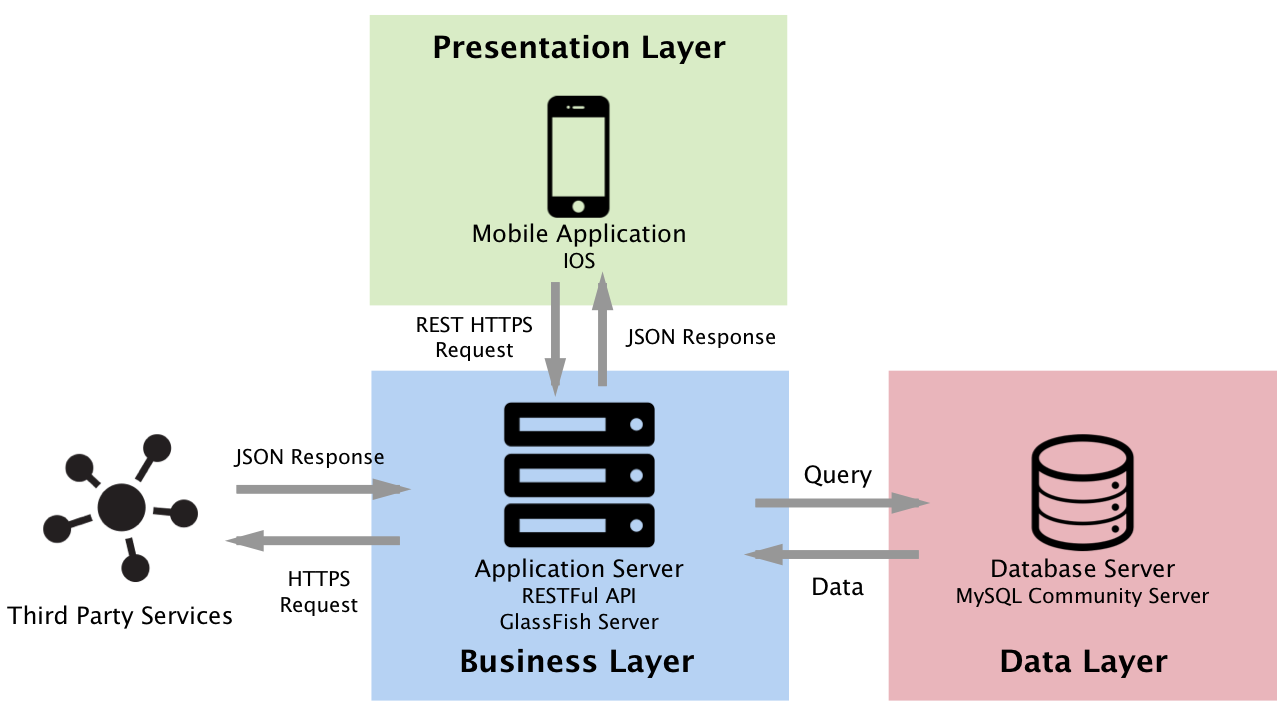
\includegraphics[scale=0.45]{highLevelView.png}
    \caption{High Level View of the system's architecture}
    \label{fig:highLevelView}
\end{figure}
The \textbf{Presentation Layer} is the most external layer of the system, and is responsible for handling all GUI communication and logic. This layer does not handle data or process business rules, but it forwards all the requests to the layers bellow and translates the system operations results of these requests to something that users can understand. It is the only layer of the system that users can access directly and interact with.

The \textbf{Business Layer} implements all core functionality of the system. It's in this layer that the application logic and business rules are implemented, in particular, all the operations related to a user account and the appointment creation and management are performed by components of this layer. This layer interacts with the APIs exposed by the Data Layer in order to store and retrieve data. The business layer also depends on some third party systems and the external services they provide (specifically for the implementation of the appointment creation and management and travel mean functionality). These external services are directly invoked by some of the classes of the Business Layer using a public API provided by those.

At last, the \textbf{Data Layer} is the lowest layer of the architecture and includes the data persistence mechanisms responsible for data storage and management. It also provides an API to the Business Layer that exposes methods of managing the stored data without creating dependencies on the data storage mechanisms, promoting the encapsulation of the persistence mechanisms and avoiding data exposition. 

Even though the \textbf{Third Party Services} don't belong to any particular layer, these services are illustrated in the figure above in order to highlight that the interaction with these will happen at the level of the Business Layer.
\subsection{Component View}
The main function of this section is to present a more detailed description of the components that must be developed as part of Travlendar+.

In the following diagram, we can see the component view of the system (the more complex components will be analyzed in further detail).
\begin{figure}[H]
    \centering
    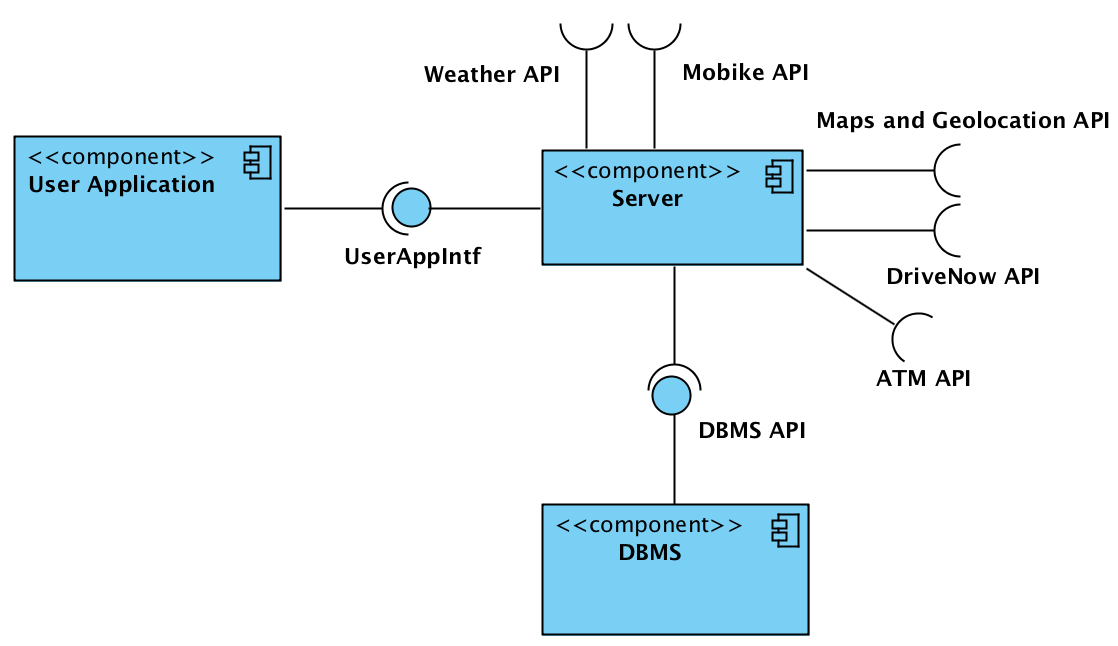
\includegraphics[scale=0.45]{componentView.png}
    \caption{Component Diagram of the system}
    \label{fig:componentView}
\end{figure}
The \textbf{User Application} is the component responsible for providing the user interfaces that allow the user to interact with the system and all of its functionality. Since a thin-client architecture is being used to implement a client/server architecture, the bulk of the data processing occurs on the server. Given this, the User Application component will act as a simple "terminal" to send requests to the server, being therefore quite simple and not needed to go into further detail.

The \textbf{Server} is the main component of the system, responsible for the data processing in order to provide all of the system's functionality. Given its complexity, it will be analyzed in further detail later in this section.

The \textbf{Database Management System (DBMS)} is the component responsible for storing and retrieving data in a persistent and reliable way. Instead of implementing this component from scratch, a commercial solution shall be used (MySQL for example).

\subsubsection{Server detailed analysis}
Being the most complex component of the system, it is useful to analyze in detail the Server's constitution.

As mentioned previously, this component is primarily responsible for all operations related to system functionality. More specifically, this component is divided into six sub-components, each related to a different kind of functionality and operations:
\begin{figure}[H]
    \centering
    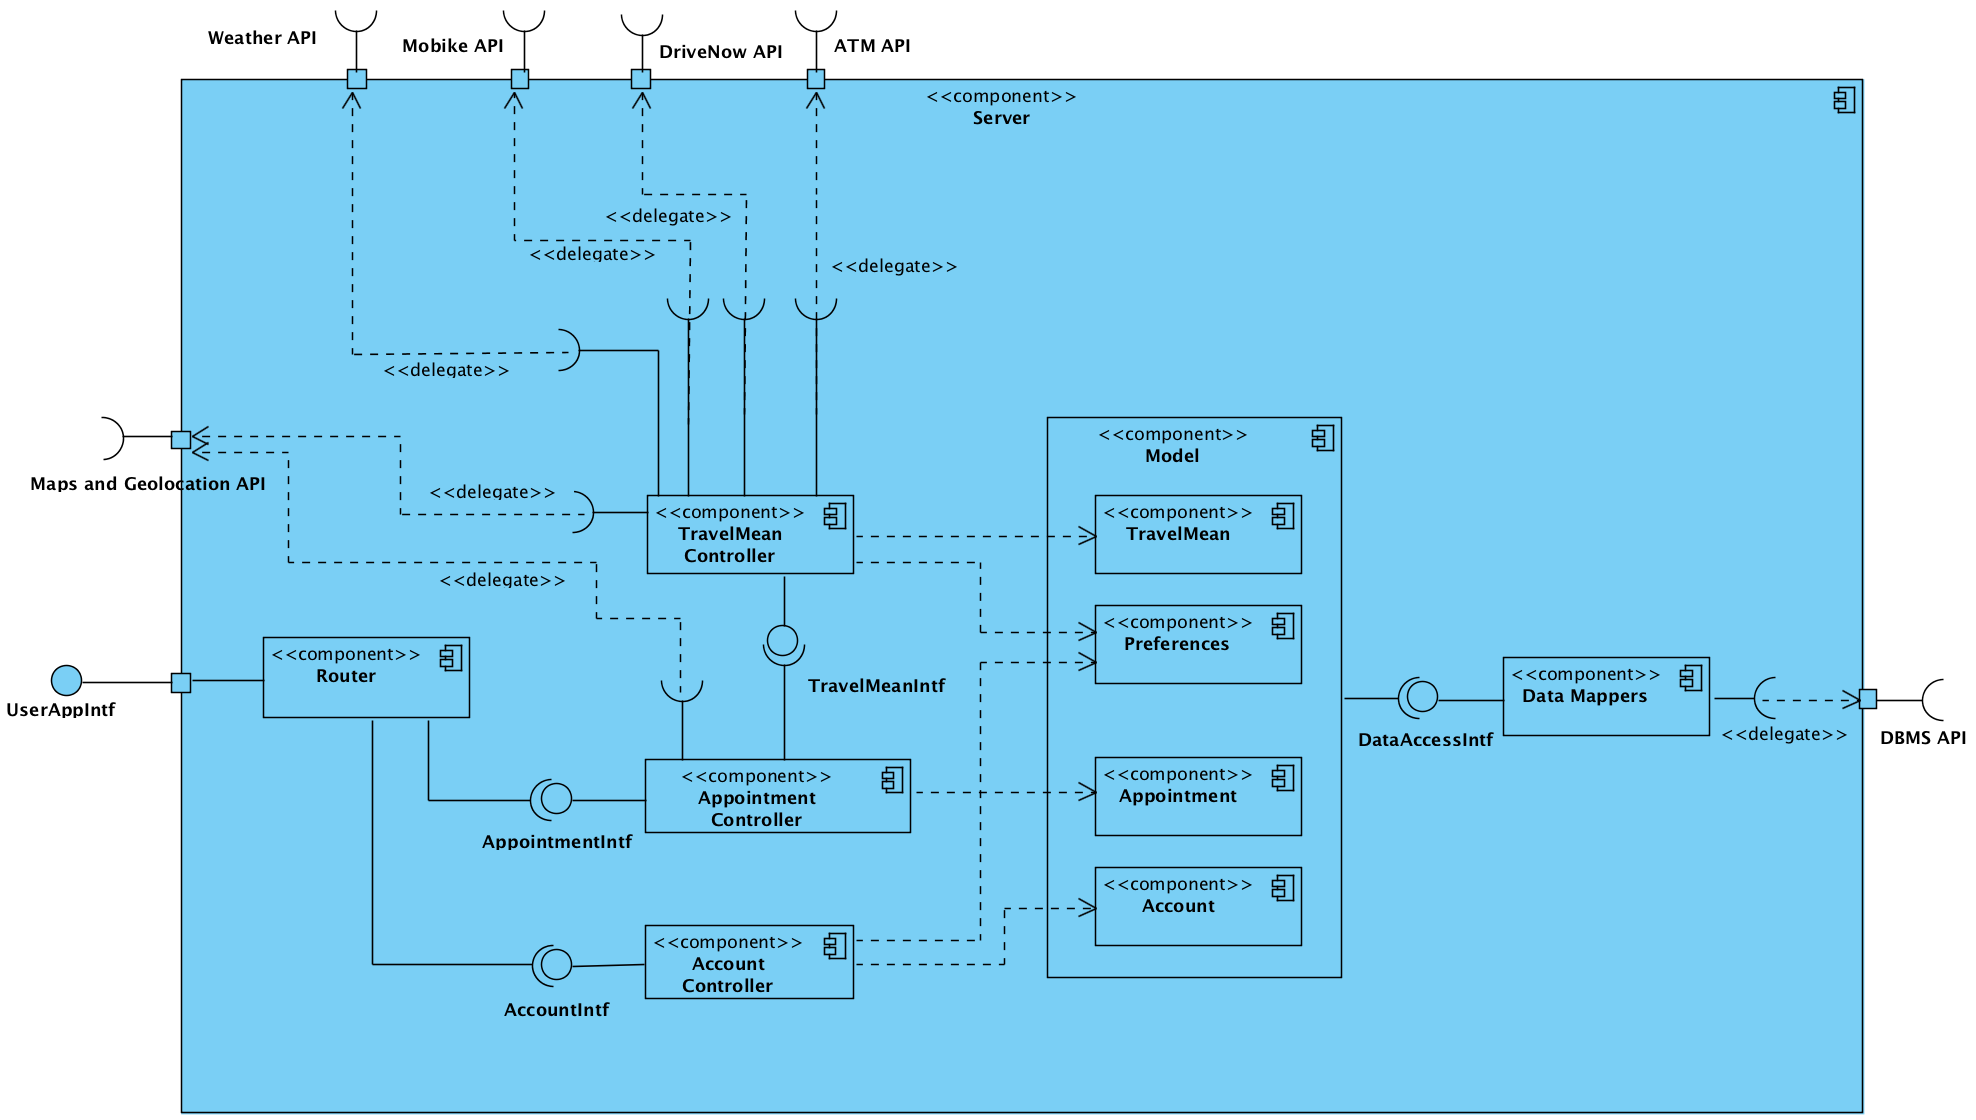
\includegraphics[scale=0.426]{serverComponentView.png}
    \caption{View of Server Component in detail}
    \label{fig:componentView}
\end{figure}
\begin{itemize}
    \item The \textbf{Router} sub-component receives the requests from the User Application and forwards (routes) them to the corresponding controller.
    \item The \textbf{Travel Mean Controller} sub-component performs all the necessary operations to compute the best travel means to get to an appointment, given the schedule at that time. This module is the one with more external interfaces since it needs to gather data from the transport services and weather services in the city of Milan in order to perform its functions.
    \item The \textbf{Appointment Controller} sub-component performs all the necessary operations that allow the user to create, edit and delete an appointment. It is also responsible for all the needed procedures that allow the user to always have the best possible schedule: schedule and arrange the appointments according to the parameters the user defines for each appointment and based on the time the user needs to get from one appointment to another (data computed by the Travel Mean Controller, which explains the interface to this component). This, allied with the Travel Mean Controller, fulfills all the requirements related to the appointment creation and managing.
    \item The \textbf{Account Controller} sub-component implements all the methods for inserting or updating information about the users. More specifically, it allows the creation of new users (registration of visitors) and login of already existing users. It also performs all the necessary operations to allow the user to edit all of his preferences related to the travel means.
    \item The \textbf{Model} sub-component (and all of its sub-components) manages the behavior and data of the application domain and responds to requests or instructions by the respective controller.
    \item The \textbf{Data Mappers} sub-component is a layer of software which separates the model from the database and acts as a "middle-man" for the interactions between these two.
\end{itemize}


\subsubsection{Database detailed analysis}
The following ER provides a graphical representation of the conceptual model of the database.

\begin{figure}[H]
    \centering
    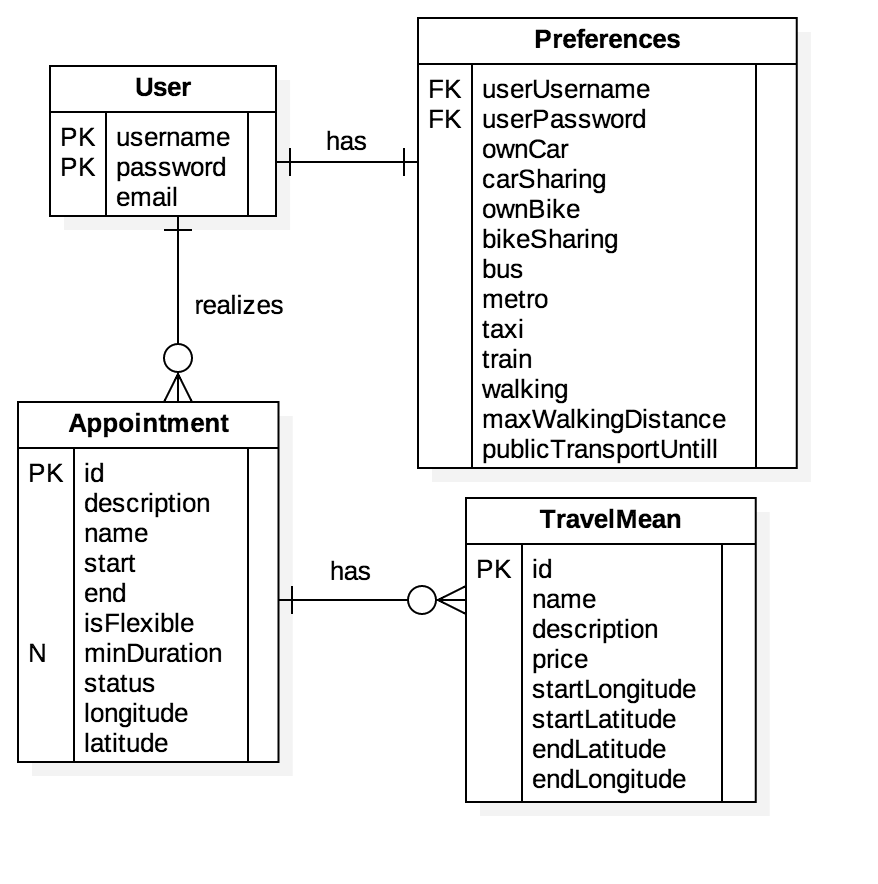
\includegraphics[scale=0.30]{databaseER.png}
    \caption{Database ER}
    \label{fig:databaseER}
\end{figure}

\subsection{Deployment View}
The main purpose of this section is to show how the software components described above are going to be deployed in the system's hardware infrastructures. This characteristic makes the developer's task easier since the mapping between software and hardware becomes explicit.

\begin{figure}[H]
    \centering
    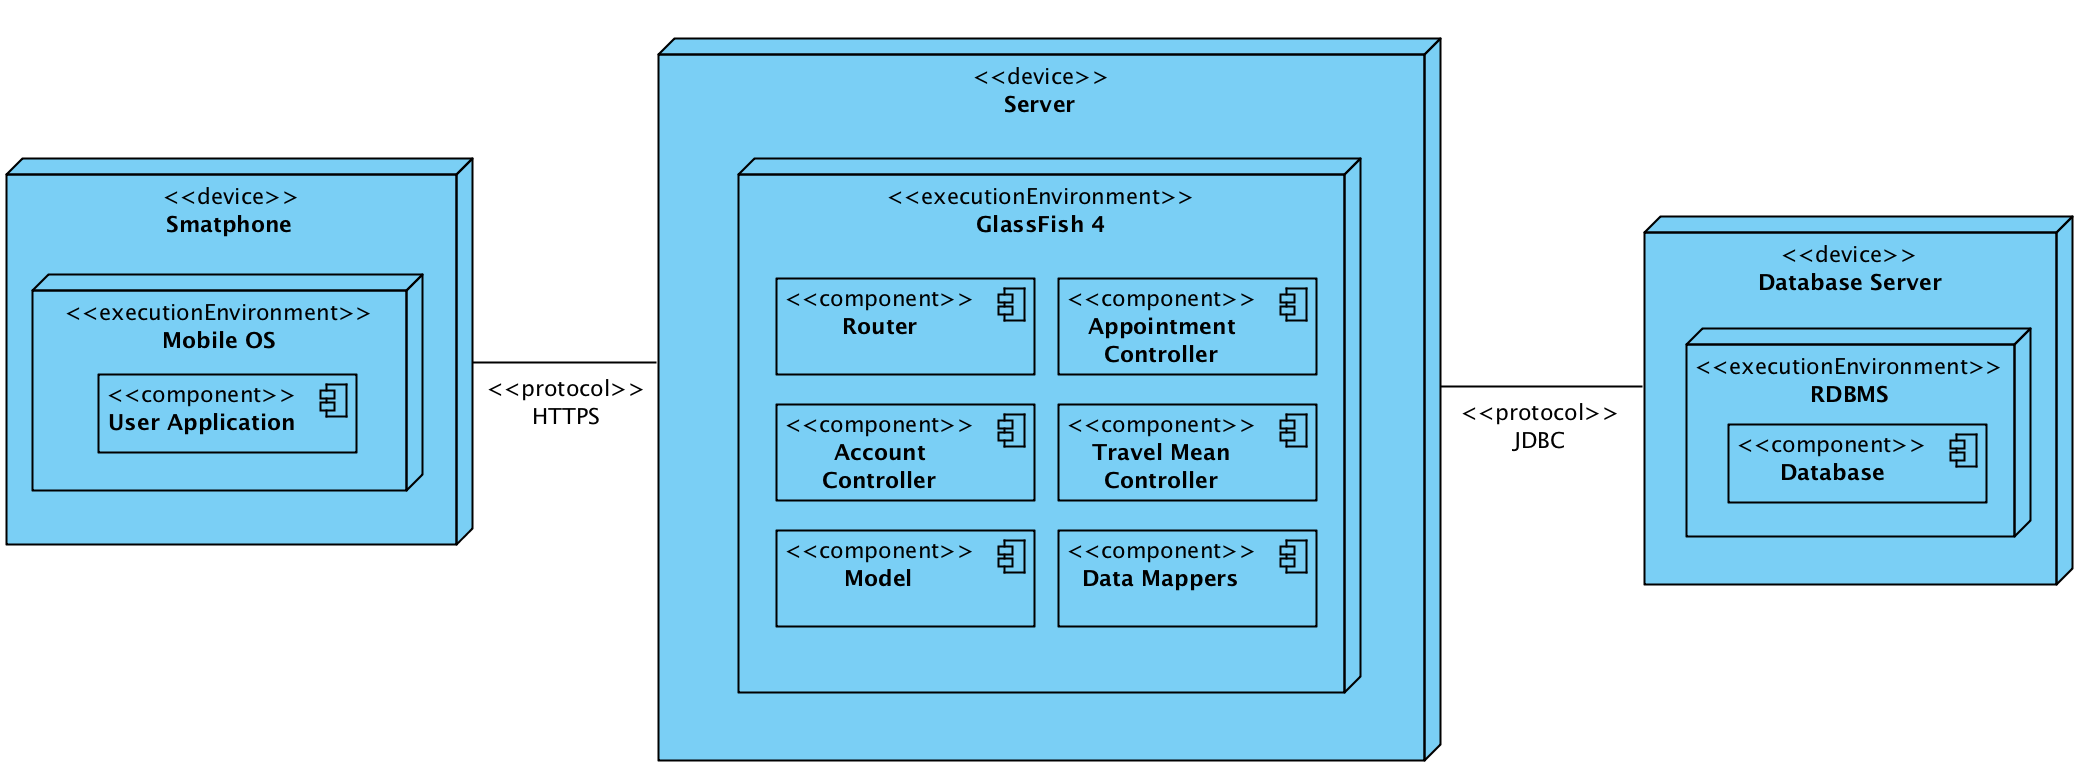
\includegraphics[scale=0.41]{deploymentView.png}
    \caption{Deployment View of the system}
    \label{fig:componentView}
\end{figure}


\subsection{Runtime View}
The following diagrams are intended to describe the interactions between the main system components when performing a sample amount of functionality. These diagrams are still a high-level view of the system, since the function names or even the functions themselves may change during the development process.
\subsubsection{User Login}

\begin{figure}[H]
    \centering
    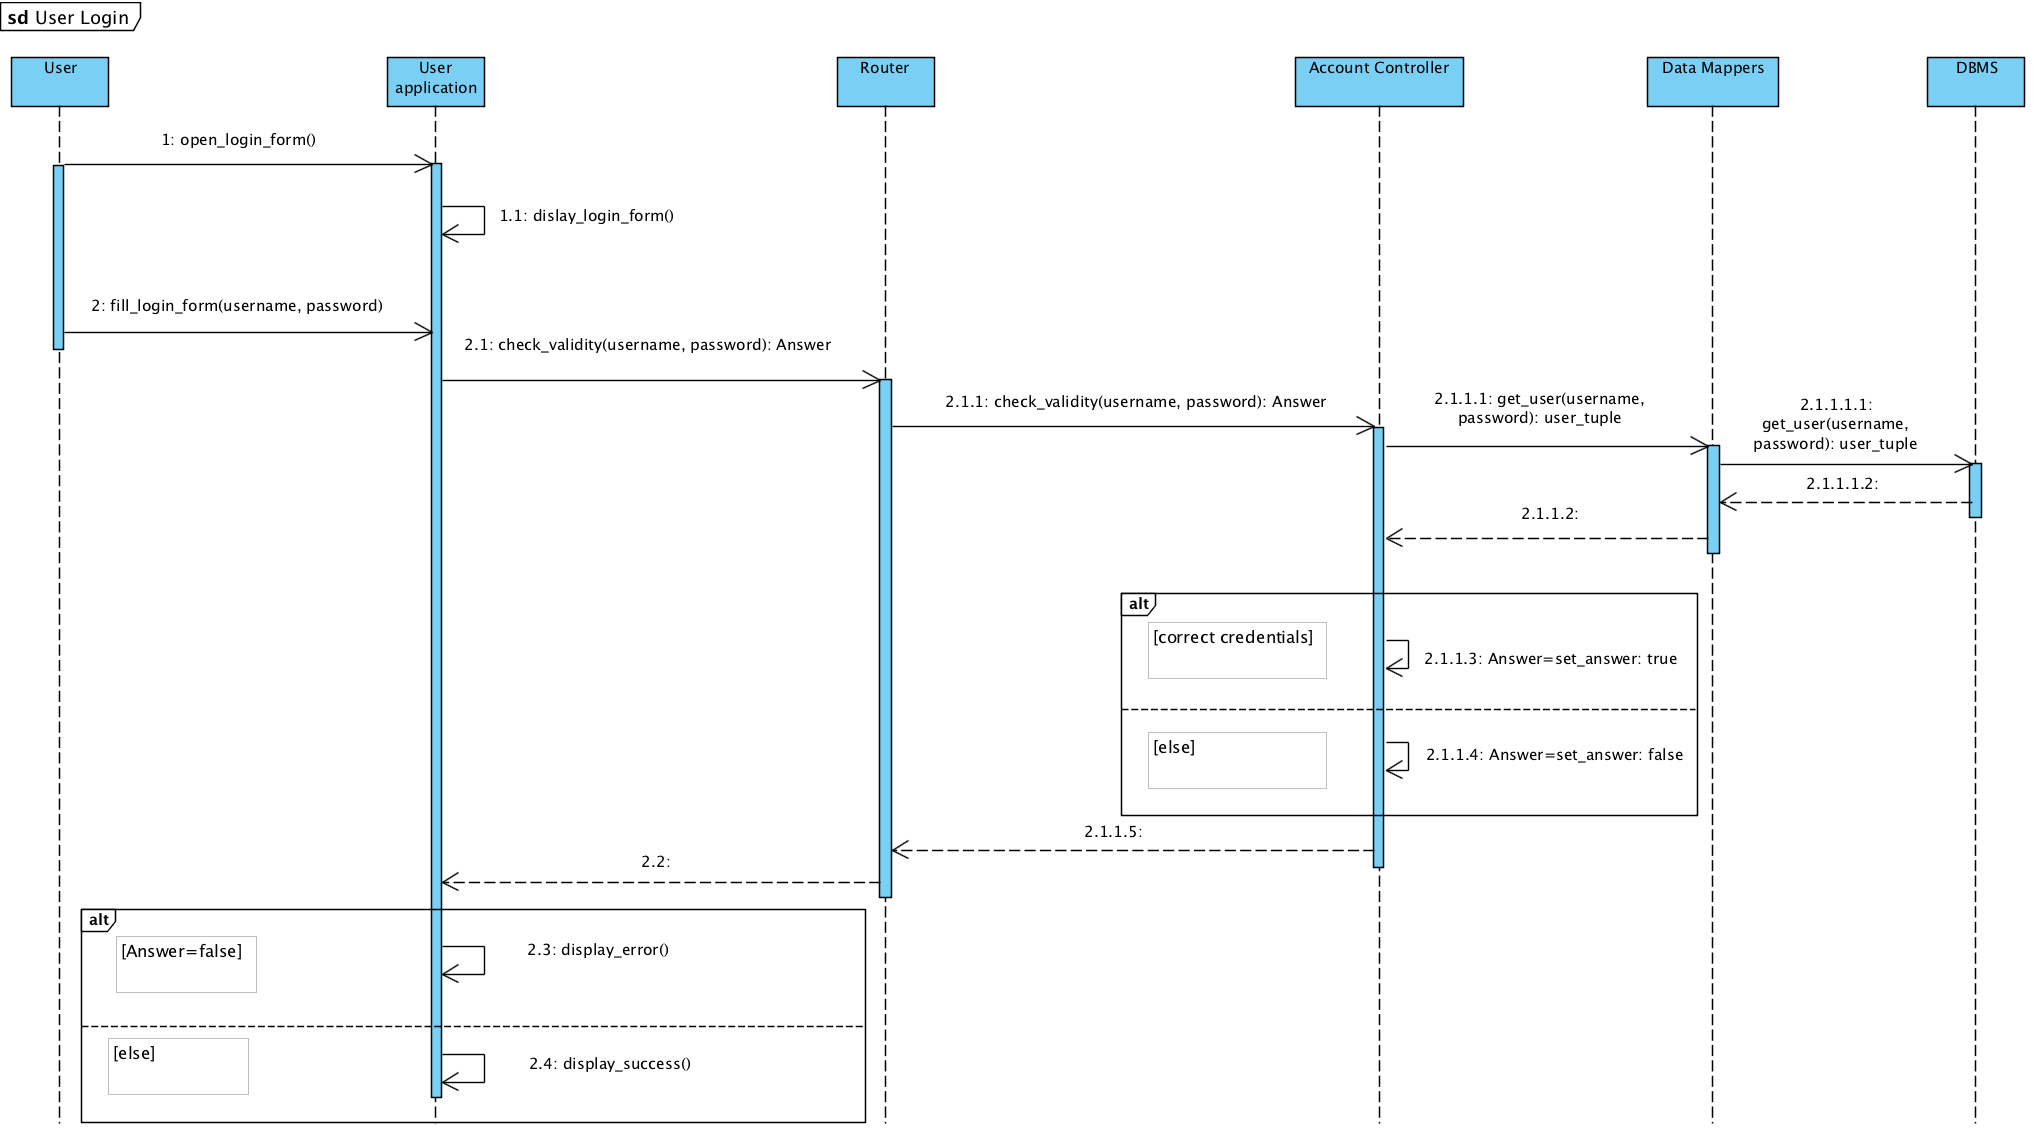
\includegraphics[scale=0.48, angle=-90, origin=c]{loginRuntimeView.png}
    \caption{User Login}
    \label{fig:loginRuntime}
\end{figure}

\subsubsection{Create Appointment}

\begin{figure}[H]
    \centering
    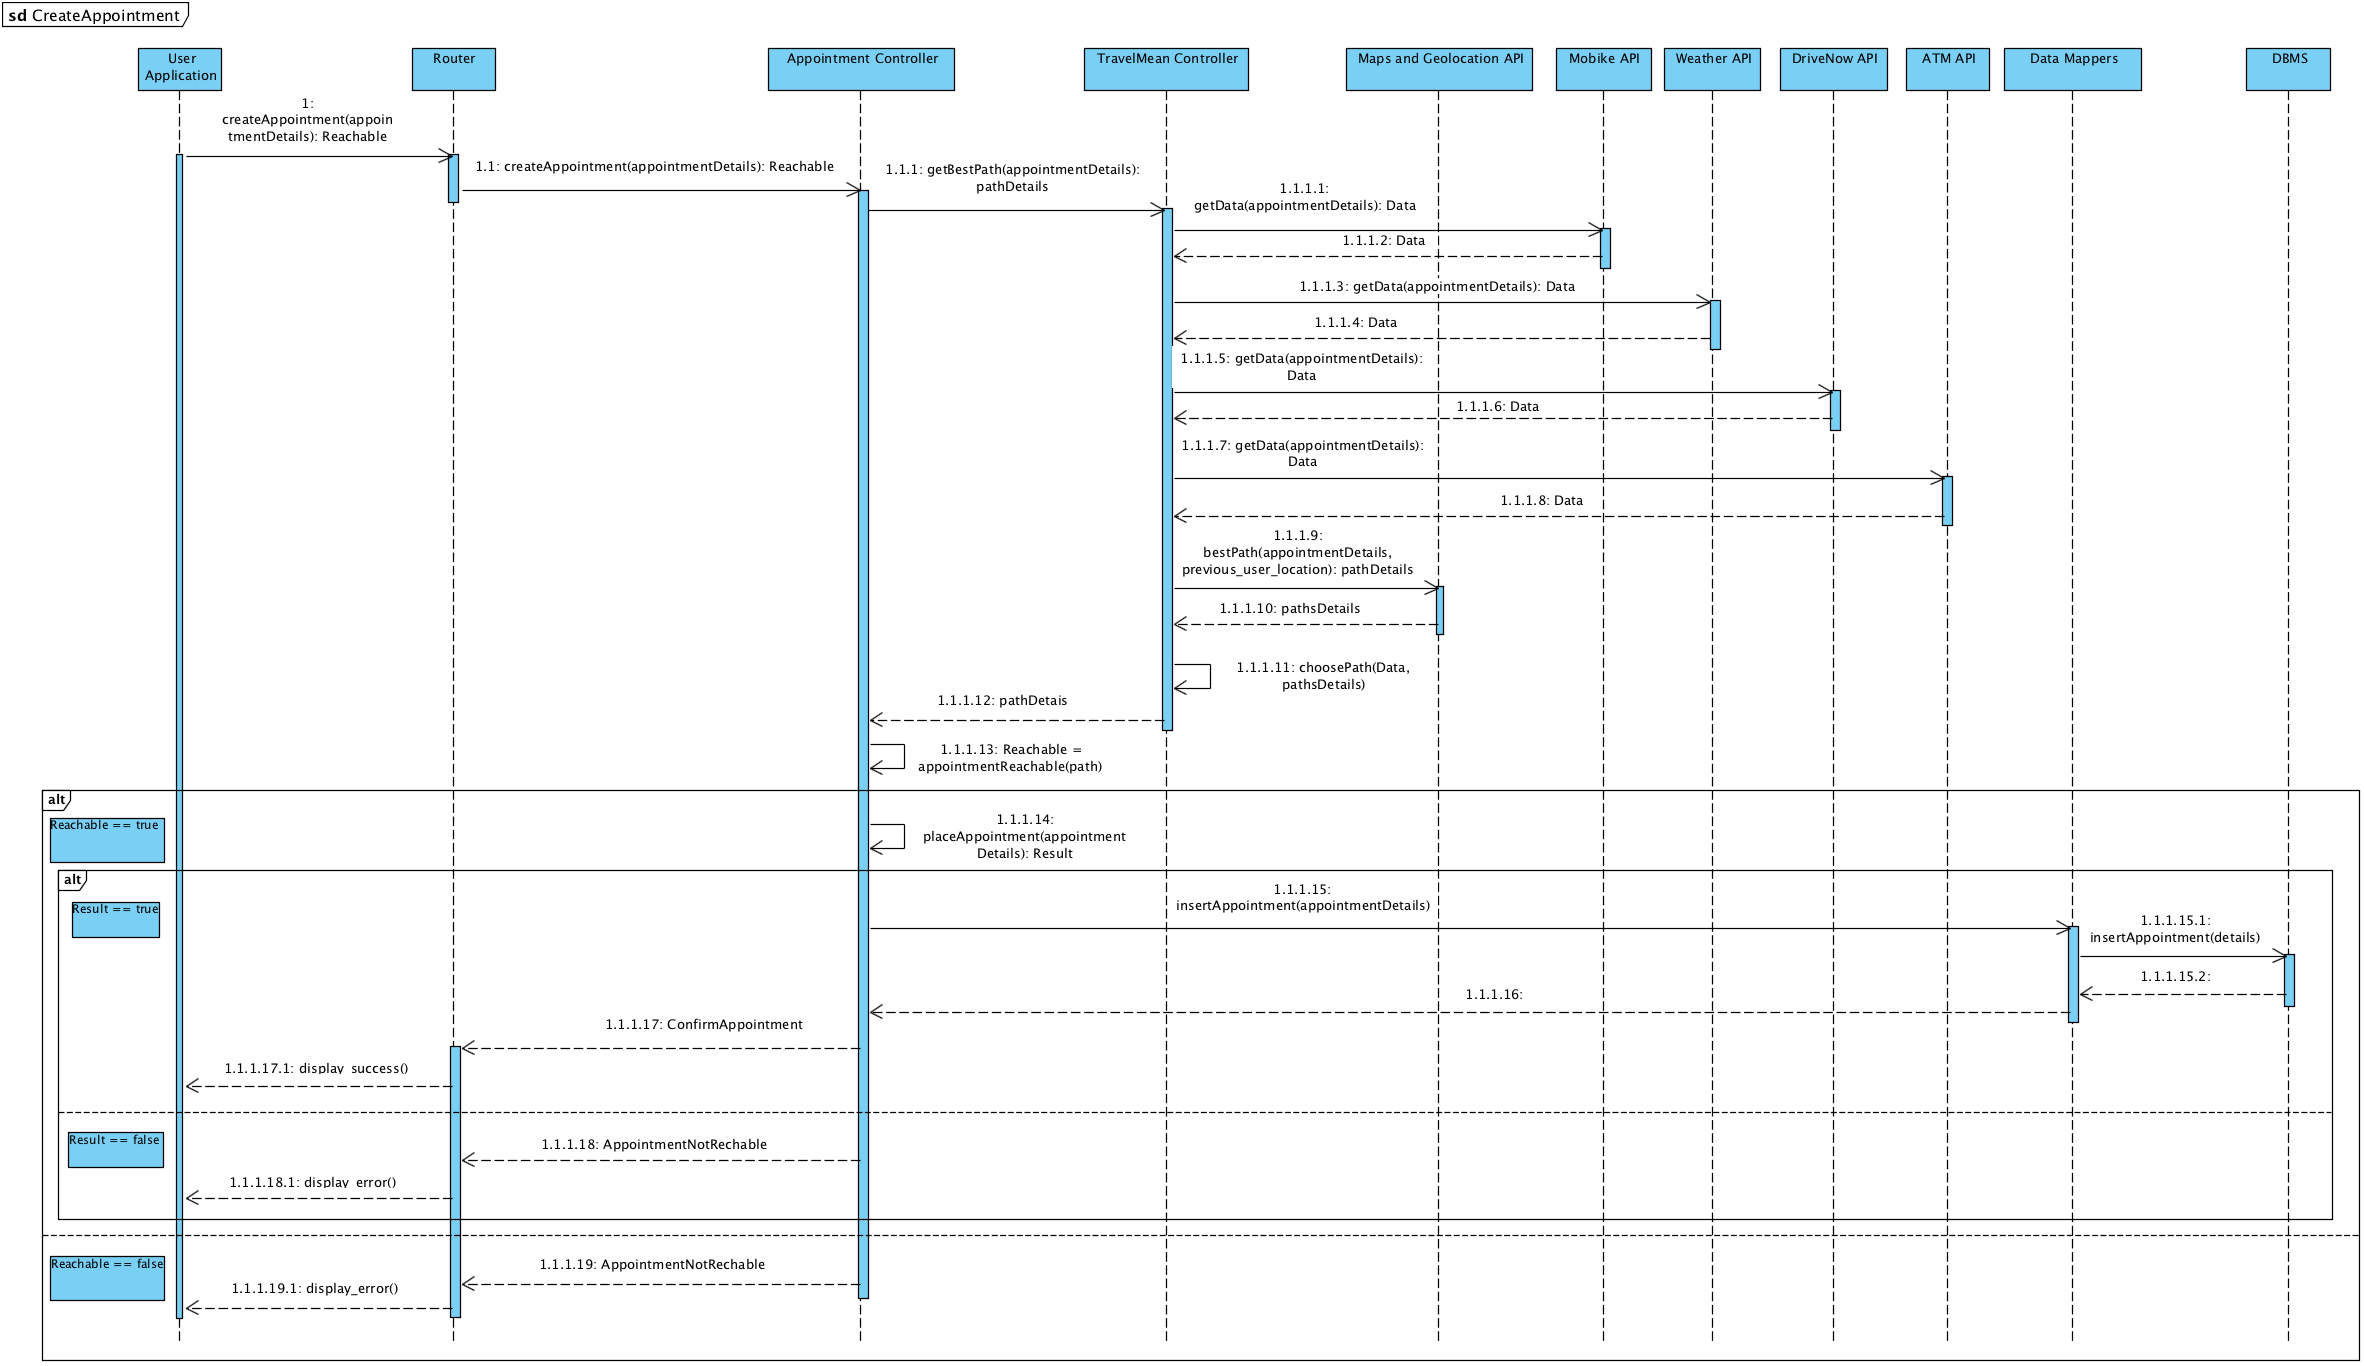
\includegraphics[scale=0.45, angle=-90, origin=c]{appointmentRuntimeView.png}
    \caption{User Appointment Creation}
    \label{fig:appointmentRuntime}
\end{figure}

\subsubsection{Change Preference}

\begin{figure}[H]
    \centering
    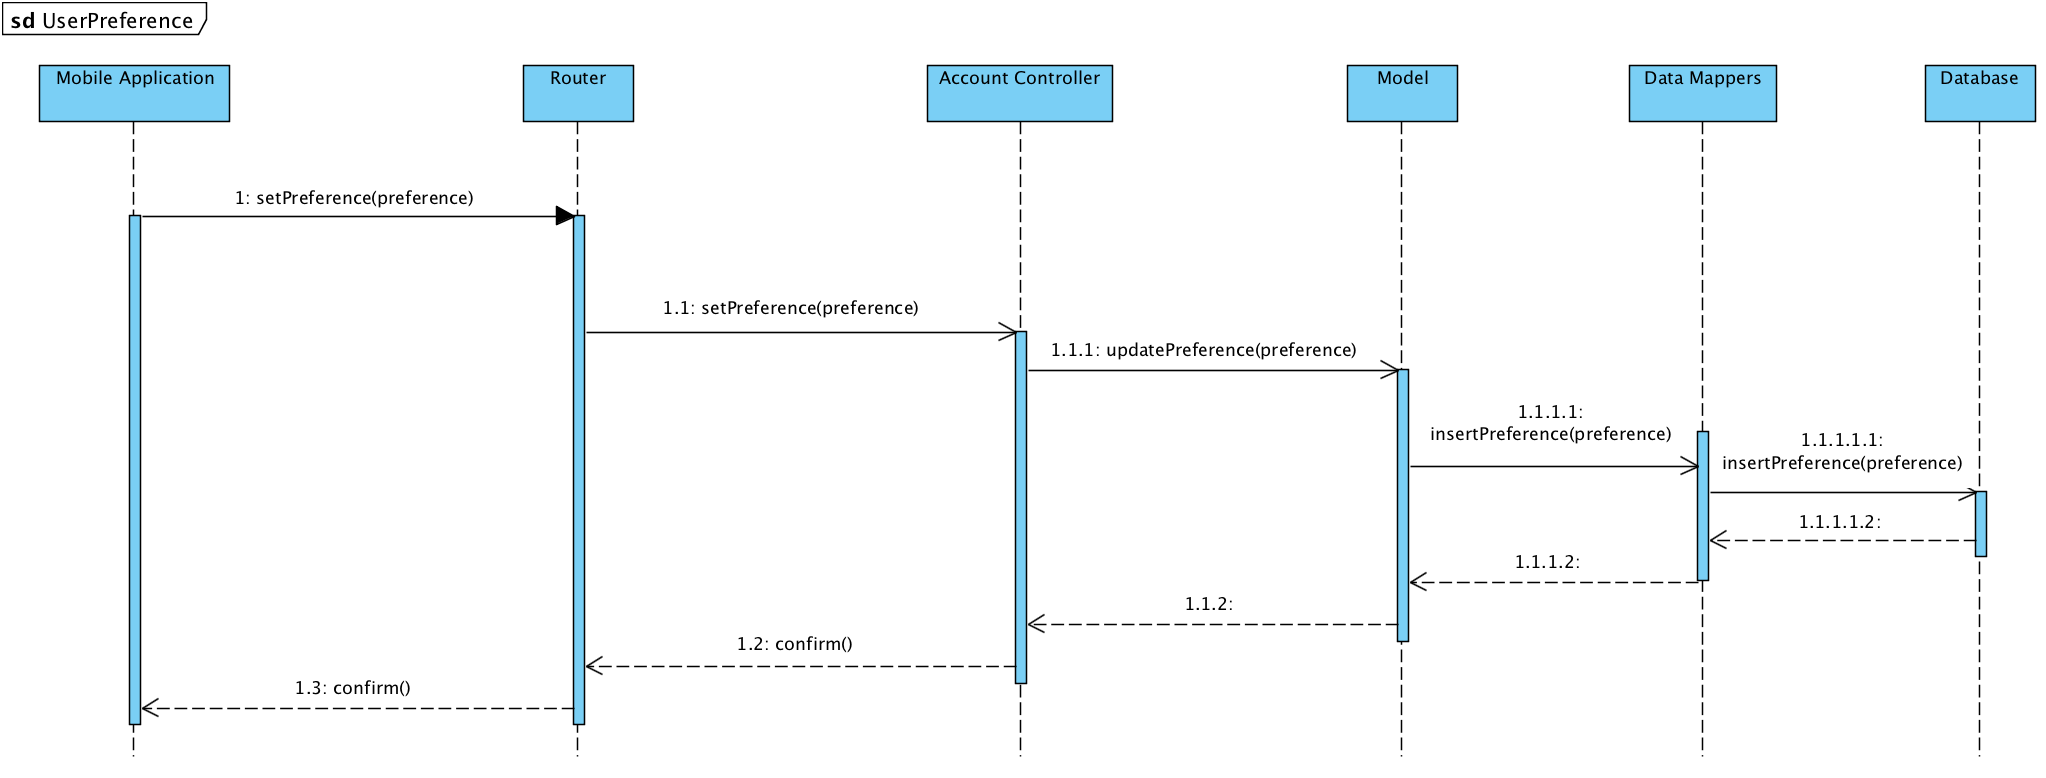
\includegraphics[scale=0.48, angle=-90, origin=c]{preferenceRuntimeView.png}
    \caption{Change Preference}
    \label{fig:preferenceRuntime}
\end{figure}

\subsection{Component Interfaces}
In this section the interfaces through which the different system's components interact will be described, and so will the main methods associated with each interface
\begin{itemize}
    \item The \textbf{UserAppIntf} interface represents the way the User Application interacts with the Server, being this the only interface through which these two can communicate. This interface provides all of the methods provided by the \textbf{AppointmentIntf} and the \textbf{AccountIntf}.
    \item The \textbf{AppointmentIntf} interface represents the way components can interact with the Appointment Controller, responsible for managing all of the aspects associated with the appointment management. This interface provides the following methods:
    \begin{itemize}
        \item createAppointment(string: name, string: description, date: from, date: to, float: longitude, float: latitude): receives the necessary data to create an Appointment and creates it.
        \item createFlexibleAppointment(string: name, string: description, date: from, date: to, time: minDuration float: longitude, float: latitude): receives the necessary data to create a Flexible Appointment and creates it.
        \item editAppointment(int: appointmentId, data): receives the data parameters related to an appointment that are supposed to be changed and the id of that appointment. The data parameters are the ones described above.
        \item deleteAppointment(int: appointmentId): deletes the appointment that matches the appointment Id.
        \item checkReachibility(appointmentDetails): checks if the appointment to be created/edited is reachable or not.
    \end{itemize}
    \item The \textbf{AccountIntf} interface represents the way components can interact with the Account Controller, responsible for managing all of the aspects associated with the user account. This interface provides the following methods:
    \begin{itemize}
        \item createAccount(string: username, string: email, string: password): registers a visitor into the system, creating an account for him.
        \item loginUser(string: username, string: password): logs a user into the system.
         \item recoverPassword(string: email): sends a new password to the user email, deleting the previous one.
        \item setPreference(string: newPreference): changes a user preference to its new value.
    \end{itemize}
    \item The \textbf{TravelMeanIntf} interface represents the way components can interact with the Travel Mean Controller, responsible for managing all of the aspects associated with the travel means used to get to the appointments. This interface provides the following methods:
    \begin{itemize}
        \item getBestPath(appointmentDetails): receives the data parameters related to the appointment in question and returns the best travel mean to get to that appointment.
    \end{itemize}
    \item The \textbf{DataAccessIntf} interface represents the way components can interact with the Data Mappers Component. It provides all of the needed methods and mechanisms to abstract the interaction between the database and the system.
    \item The \textbf{Maps and Geolocation API} interface represents the way components can interact with the Maps and Geolocation service. It provides all the needed methods to get information about the appointment location and the best routes and travel means to get to that location.
    \item The \textbf{Weather API} interface represents the way components can interact with the Weather Service. It provides all the needed methods to get information about the weather forecast in a specific place and time.
    \item The \textbf{Mobike API} interface represents the way components can interact with the Mobike service. It provides all the needed methods to get information about the bicycle's location and cost.
    \item The \textbf{DriveNow API} interface represents the way components can interact with the DriveNow service. It provides all the needed methods to get information about the cars location, status, and cost.
    \item The \textbf{ATM API} interface represents the way components can interact with the ATM service. It provides all the needed methods to get information about the travel mean schedule.
    \item The \textbf{DBMS API} interface represents the way components can interact with the Database. This interface provides the usual methods that are needed to interact with a database, like update, insert, delete and select queries.
\end{itemize}


\subsection{Selected architectural styles and patterns}

\subsubsection{Client/Server Architecture} This architectural style keeps all the logic of the program, which is computationally heavy, on the server side, while the end-users only need to offer a simple amount of presentation functionality. This allows the system to be centralized, improving:
\begin{itemize}
    \item Performance: system's files are only accessed by the server, so they're all in the same place, becoming easier to manage and faster to access
    \item Security: facilitates the implementation of security layers and protocols between the client and the server, setting up access rights to reach the server for example
    \item Scalability: it's easy to change the logic server-side without any implication on the client side
\end{itemize}

\subsubsection{Service Oriented Architecture} This architectural pattern allows the system to be designed as a collection of services that communicate with each other. This way, the external APIs that the system interacts with can be interpreted as a set of these services, which makes them easily implementable (in this case our system is the service consumer, and the APIs are the service providers). It is also possible to see our system as the service provider, first providing an initial set of services and eventually, with the addition of some additional components, increasing the number of services provided.

\subsubsection{Layered Architecture} This architectural pattern promotes a great level of separation of concerns between the various components of the system, given that every component operates at a single logical layer of abstraction. This design choice also simplifies the implementation and testing phase of the system: since the layers are isolated from each other, it is possible to test a specific layer even if the underlying layers aren't implemented, using mocks or stubs to simulate the functionality of those.

\subsubsection{3-Tier Physical Architecture} This architectural style allows the various components of the system to be deployed on different devices, given the decoupling that exists between the modules. It also allows for any of the three tiers to be upgraded or replaced independently in response to changes in requirements or technology, improving the system's scalability. The system will be composed of 3 tiers: Presentation tier, Business tier (the business logic of the system) and Data tier.

\subsubsection{Model-View-Controller} This architectural pattern divides a given application into 3 interconnected parts, separating the internal representation of information from the way this information is presented to the user. This is one of the most used patterns to promote decoupling between the major components of a system, allowing for efficient code reuse and parallel development.

\subsubsection{Remote Facade} This architectural pattern provides a unified interface to a set of interfaces in a subsystem. Facade defines a higher-level interface that makes the subsystem easier to use. Given that the communication between the different components of our system will happen over the network, the existence of a Facade with coarse-grain methods that map to various fine-grained ones also improves the communication's efficiency (fewer packets have to be sent over the network). With all this, it promotes decoupling between the server and the user application, since all the remote calls are made through one interface and then mapped inside the server (by the router component) to the respective controller.

\subsubsection{Data Mapper} This architectural pattern is a data source architectural pattern. It consists of a layer of software that separates the domain layer objects from the database. Its responsible for transferring data between the two while keeping them isolated from each other and from the mapper itself.

\subsubsection{REST} A REST architectural style with JSON data model format is also being used to allow the communication between the User Application and the Server, being this based on HTTP requests (POST, GET, PUT and DELETE to name the most important ones).

\subsubsection{Other design decisions}
\begin{itemize}
    \item \textbf{Application Server:} GlassFish 4.1 was chosen since it provides containers for both the EJB and the JSP pages, and is a full Java EE Application server.
    \item \textbf{DMBS:} MySQL was chosen as DBMS since it's free and one of the most popular DBMS, with a big community and lots of documentation.
\end{itemize}

\section{Algorithm Design}
In this section, it is presented an overall description of the most relevant algorithms for the Travlendar+ system, explained using pseudo-code notation.


\subsection{Appointment Placement Algorithm}
The first and second algorithms check if it is possible to insert a new Fixed Appointment and a new Flexible Appointment, respectively, in the user's schedule and, if possible, inserts it.

\subsubsection{Fixed Appointment Placement Algorithm}

If this new appointment is a fixed one, there are three possible situations:
\begin{itemize}
    \item The time interval of the appointment is free - the new appointment is successfully inserted in the system
    \item The time interval of the appointment isn't free, but the system manages to reschedule an adjacent flexible appointment, leaving enough space for this appointment to be scheduled - the new appointment is successfully inserted in the user's schedule.
    \item There is no way of inserting that appointment into the user's schedule - the system returns an error message.
\end{itemize}

\begin{algorithm}[H]
\SetAlgoLined
\Begin{
    $N\leftarrow New Fixed Appointment$\;
        \uIf{$N_{timeInterval}=free$}{
            $insert(N)$\;
            $return\ True$\;}
        {\uIf{$Flexible Appointments In (N_{end}-N_{start})=1$}{
        
            \uIf{$Flexible Appointment\ before\ N_{start} $ {\bf and} $Previous Fixed Appointment_{end}-N_{start} > Flexible Appointment_{minDuration} + TimeToGetToFlexibleAppointment + TimeToGetToN$ {\bf and} $possibleInterval(Flexible Appointment, Previous Appointment_{end}, N_{start})$}{
            $relocate(Flexible Appointment)$\;
            $insert(N)$\;
            $return\ True$\;}
            
            \uElseIf{$Flexible Appointment\ after\ N_{start} $ {\bf and} $Next Fixed Appointment_{start}-N_{End} > Flexible Appointment_{minDuration} + TimeToGetToFlexibleAppointment + TimeToGetToNextFixedAppointment$ {\bf and} $possibleInterval(Flexible Appointment, N_{end}, Next Appointment_{start})$}{
            $relocate(Flexible Appointment)$\;
            $insert(N)$\;
            $return\ True$\;}
        }
        \uElseIf{$Flexible Appointments In (N_{end}-N_{start})=2$}{
        
            \uIf{$Flexible Appointment1\ before\ N_{start} $ {\bf and} $Previous Fixed Appointment_{end}-N_{start} > Flexible Appointment1_{minDuration} + TimeToGetToFlexibleAppointment + TimeToGetToN$ {\bf and} $possibleInterval(Flexible Appointment1, Previous Fixed Appointment_{end}, N_{start})$ {\bf and} $Flexible Appointment2_{start}\ after\ N_{end} $ {\bf and} $NextFixe Appointment_{start}-N_{end} > Flexible Appointment_{minDuration} + TimeToGetToFlexibleAppointment + TimeToGetToNextAppointment$ {\bf and} $possibleInterval(Flexible Appointment, N_{end}, Next Appointment_{start})$}{
            $relocate(Flexible Appointment1)$\;
            $relocate(Flexible Appointment2)$\;
            $insert(N)$\;
            $return\ True$\;}
            
        }
        $return\ False$
        
    }
}
\caption{Fixed Appointment Placement}
\end{algorithm}

\subsubsection{Flexible Appointment Placement Algorithm}

If this new appointment is a flexible one, there are two possible situations:
\begin{itemize}
    \item There is a free space in the user's schedule that fits the given appointment time interval and is at least as big as the flexible appointment's minimum duration plus the time to get there - the new appointment is successfully inserted in the system.
    \item There is no way of inserting that appointment into the user's schedule - the system returns an error message.
\end{itemize}

\begin{algorithm}[H]
\SetAlgoLined
\Begin{
    $N\leftarrow New Flexible Appointment$\;
        \uIf{$N_{timeInterval}=free$}{
            $insert(N)$\;
            $return True$\;}
        {\uIf{$Fixed Appointments In (N_{end}-N_{start})$}{
        
            \uIf{$AppointmentAfter_{start} - AppointmentBefore_{end} > N_{minDuration} + TimeToGetToN + TimeToGetToAppointmentAfter $}{
                $insert(N)$\;
                $return\ True$\;
            }
        }
        $return False$\;
        
    }
}
\caption{Flexible Appointment Placement}
\end{algorithm}

\subsection{Reachability Checker Algorithm}
This third algorithm checks if an appointment is reachable or not. Given a schedule state and a new appointment to be inserted, it computes the time interval between the previous appointment end time and the starting time of the appointment to be inserted and, if this interval is smaller than the required time to get from the previous location to the new appointment's location, the system returns that the appointment is reachable. Otherwise, it is unreachable.

Bellow the pseudo code for this algorithm is presented, in order to better understand it:

\begin{algorithm}[H]
\SetAlgoLined
\Begin{
    $L2\leftarrow New Appointment Location$\;
    \eIf{$Previous Appointment$}{
        $L1\leftarrow Previous Appointment Location$\;
        $T1\leftarrow Previous Appointment_{endTime}$\;
    }
    {
        $L1\leftarrow User Location$\;
        $T1\leftarrow 0$
    }
    $T2\leftarrow NewAppointment_{startTime}$\;
    $\Delta T\leftarrow T2-T1$\;
    
    $T3\leftarrow Time To Get From Old Appointment To New$\;
    \eIf{$\Delta T \geq T3$}{
        $return\ True$\;}
    {$return\ False$}
    \caption{Reachability Checker}
}
\end{algorithm}

\section{User Interface Design}
\subsection{Mockups}
One of the most important things to take into consideration when designing an information system is the way its functionality is going to be provided to the user. Since the user interacts with our system through a GUI, saying this is the same as saying that this user interface has to be as simple and intuitive to use as possible.

Another thing that was taken into consideration while designing the interfaces was the adaptability of it to the different smartphone screen resolutions and form factors available on the market. To satisfy this requirement, the interface was drawn in a minimalist way, without demanding animations and small details that would make it impossible to use on smaller screens with low resolution.

The mockups of the UI of our system can be found in \textbf{section 3.1.1 of the RASD} and were designed with all this in mind: to be as simple and intuitive to use as possible while providing to the user all of the system's functionality.

\subsection{UX Diagram}
The following UX Diagram provides additional information about the way the user interacts with the system through the mobile application, and have the purpose of complementing the UI mockups provided in the RASD document with a more "dynamic" view over the interface.

\begin{figure}[H]
    \centering
    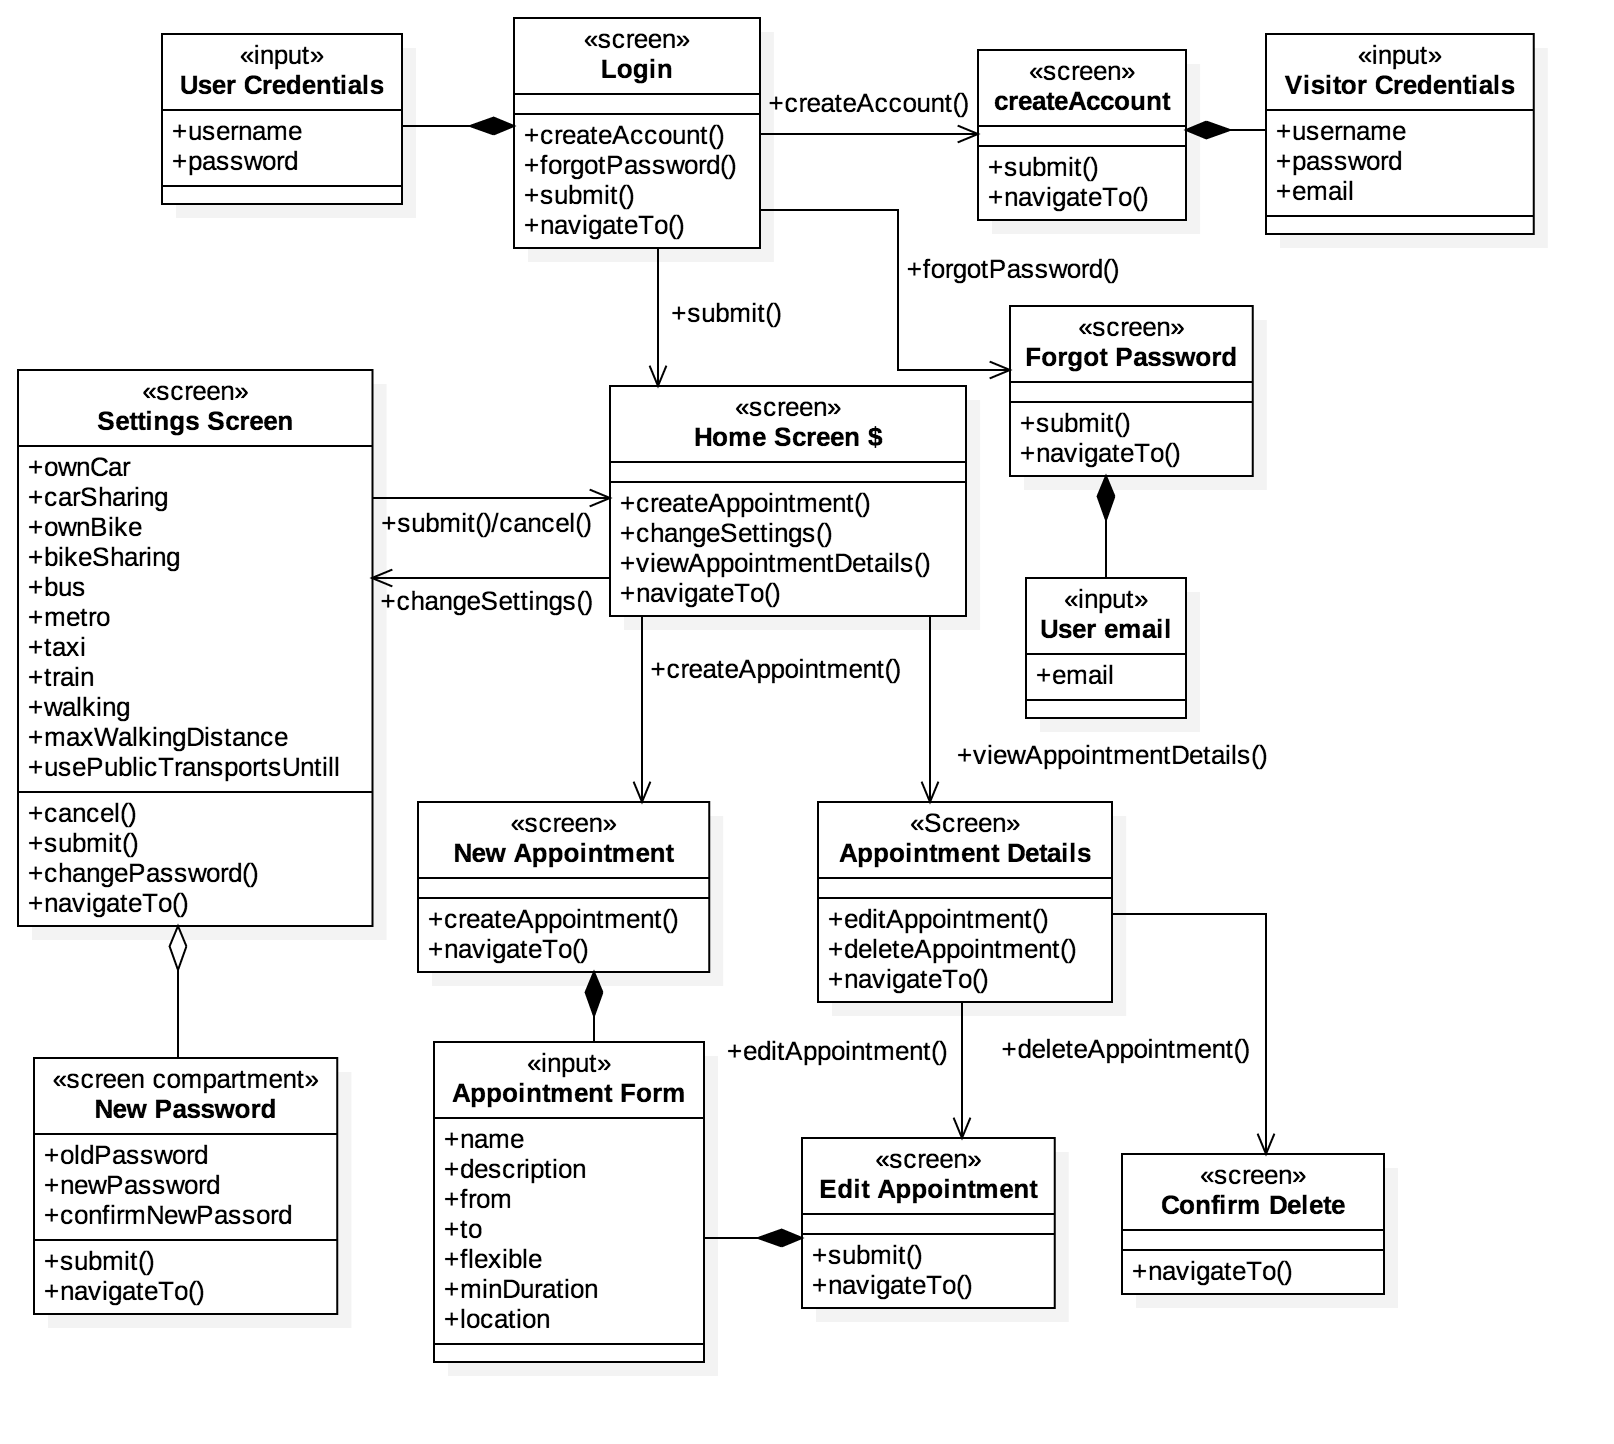
\includegraphics[scale=0.26]{uxDiagram.png}
    \caption{UX Diagram}
    \label{fig:uxDiagram}
\end{figure}

\section{Requirements Traceability}
\subsection{Functional Requirements}
All of the design choices presented in this document were made with the goals and requirements defined in the RASD in mind, and aim to fulfill them in the best possible way. The following list provides an accurate mapping between the system's goals and requirements defined on the RASD and the system components, defined in the DD, that aim to fulfill those goals and requirements.\\
\textbf{N.B.: All the requirement intervals include the first and the last on the interval.}

\begin{itemize}
    \item \textbf{{[G1]}} Allow only registered users to access the most relevant functionality of the system (R1-R4).
    \begin{itemize}
        \item The \textbf{Account Controller}, which provides the visitors the ability to register as users of the system.
    \end{itemize}
    \item \textbf{{[G2]}} Allow a logged user to create an appointment (R5-R10).
    \begin{itemize}
        \item The \textbf{Appointment Controller}, which provides all of the business logic related to the appointments management, more specifically the ability to create a new appointment.
        \item The \textbf{Travel Mean Controller}, which communicates with the third party services the system uses and implements all of the needed logic to compute for the best travel means to get to an appointment.
    \end{itemize}
    \item \textbf{{[G3]}} Allow a logged user to edit an appointment (R6-R7 and R11-R13).
    \begin{itemize}
        \item The \textbf{Appointment Controller}, which provides all of the business logic related to the appointments management, more specifically the ability to edit a previously created appointment.
        \item The \textbf{Travel Mean Controller}, which communicates with the third party services the system uses and implements all of the needed logic to compute for the best travel means to get to an appointment.
    \end{itemize}
    \item \textbf{{[G4]}} Allow a logged user to delete an appointment (R14).
    \begin{itemize}
        \item The \textbf{Appointment Controller}, which provides all of the business logic related to an appointments management, specifically to delete an appointment from the user's schedule.
    \end{itemize}
    \item \textbf{{[G5]}} Allow a logged user to have his schedule planned in the best possible way (R15-R19).
    \begin{itemize}
        \item The \textbf{Appointment Controller}, which provides all of the back end logic related to the appointments management, more specifically to make any change in the calendar related to insertion or deletion of appointments.
        \item The \textbf{Travel Mean Controller}, which communicates with the third party services the system uses and implements all of the needed logic to compute for the best travel means to get to an appointment.
    \end{itemize}
    \item \textbf{{[G6]}} Allow a logged user to define preferences related to travel means (R20-R24).
    \begin{itemize}
        \item The \textbf{Account Controller}, which provides the visitors the ability to manage its account preferences and change them according to his personal preferences.
    \end{itemize}
\end{itemize}
For all of the requirements the \textbf{Router Component} takes part in the interaction, but only maps the User Application requests to the respective controller, not being relevant to refer to in every goal. So does the \textbf{Model Component}, the \textbf{Data Mappers Component} and the \textbf{Database Component}, since our application has to access the database (either to read or to write) every time it executes one of the main system operations/functionality.

\subsection{Non-Functional Requirements}

The non-functional requirements were no exception and were also taken into consideration when making the Design Choices for the system. In particular, this analysis will be focused on the \textbf{Performance, Reliability, Availability, Security}, and \textbf{Portability} requirements.

The usage of a 3 tier infrastructure is the key to achieve most of these requirements. This infrastructure allows us not only to achieve high levels of \textbf{Performance} (components with different hardware needs can be deployed in more powerful machines) but also satisfying levels of \textbf{Reliability} and \textbf{Availability} as, thanks to the low coupling between the different components, it allows them to be distributed over the network, possibly replicated and in different server farms (highly increasing fault tolerance).

\textbf{Security} is achieved thanks to software and hardware steps. At the software level, all interface methods check if the call parameters are valid before executing its main logic and if the caller is authorized to invoke them. The database APIs will also be protected against SQL Injection and all messages between different components of the system and external APIs will be encrypted and have unique identifiers, encrypting this way all of the critical data and preventing man-in-the-middle attacks (more specifically replay attacks).

At last, \textbf{Portability} is achieved by offering a standard web service mechanism based on JSON through the API's. This allows the system to be invoked from any platform with internet access, not restricting the system to a specific operating system, programming language or hardware brand.

\section{Implementation, Integration and Test Plan}
Implementation, Integration, and Testing are 3 different activities that must be done together in order for a project to be developed in a correct way. It will be presented in the paragraphs below a plan for the implementation, integration, and testing of the different components that, together, form our system.


The system is divided into layers, and as in a traditional layered architecture, the topmost layers depend on the lowest ones. This being said, the system must be implemented using 1 out of 3 different approaches:
\begin{itemize}
    \item Bottom-Up Approach
    \item Top-Down Approach
    \item Mix between Bottom-Up and Top-Down, which meet somewhere in the middle
\end{itemize}

The \textbf{second and third} approaches imply that a component will be implemented and tested without the need for the components that this depends on to be implemented and tested already. Although this might look like a good idea, it carries a more complex development process, since mocks would have to be built in order to test the behavior of these components after being implemented.
Taking this into consideration, the \textbf{approach chosen to develop our system was a bottom-up approach.} This way, the components which do not depend on others will be the first ones to be developed and extensively tested, followed by the ones that only depend on those, until we reach the highest layer of the system, with the components that have no other component depending on them. Thanks to this a component can be tested and integrated as soon as it's finished (or even close to being finished), allowing us to complete the development and testing phase almost in parallel.
We must also keep in mind that in order to test the integration of two components, the main features of both of them should have already been developed and the related unit tests should have been performed. 

\subsection{DBMS}
The first component to be implemented is the DBMS. It shall be implemented and then fully tested before finishing the implementation of the layer above since it has to be configured and operative in order to allow to test all of the components which need access to the database.
    
\subsection{Server}
The next set of components to be implemented and tested are the ones that belong to the Business Layer, which encapsulates the business logic of the system. This layer is composed of the Server component and all of its sub-components. 

First, we should start with the \textbf{Data Mappers} sub-component, which is the Server component that mediates the interaction between the server and the database, and only depends on the DBMS component.

After this, and following a critical-module-first approach, we should develop the \textbf{Appointment Controller and Travel Mean Controller} and the \textbf{Model components associated with this ones}. Both of this controllers require the interaction with the external services to be fully functional.

The last sub-components of the server to be developed will be the \textbf{Account Controller and Router Controller} and the \textbf{Model components associated with this ones}.

After being fully implemented, the Server component must be integrated with the DBMS component, as it needs the DBMS to work properly.

Before integration testing of the two integrated components, the used external services shall be configured and fully operative.
After this, the Server can be integrated with the DBMS and shall be extensively tested, as it is the most critical and important part of the system.

\subsection{User Application}
The final part of the system to be implemented is the User Application, the topmost layer of the architecture. Since we opted for a thin client this shall be one of the easiest and fastest steps of the development process.
When finished, it shall be integrated with the rest of the components of the system in order to test the system as a whole.


\section{Effort Spent}

\begin{center}
\begin{tabular}{ |p{0.25\textwidth}|p{0.4\textwidth}|p{0.25\textwidth}| } 
 \hline
 \textbf{DATE} & \textbf{TASK} & \textbf{HOURS} \\ 
  \hline
 08/11/2017 &  Scope, Purpose and Document Structure & 1 \\ 
  \hline
 09/11/2017 & Overview and Architectural Styles and Patterns & 3 \\
  \hline
  10/11/2017 & High Level Components description and Database Component View & 4 \\ 
  \hline
  11/11/2017 & Component View and Architectural Styles and Patterns & 3 \\ 
  \hline
  12/11/2017 & Component View and Architectural Styles and Patterns & 1,5 \\ 
  \hline
  13/11/2017 & Component View and Deployment View & 4 \\ 
  \hline
  14/11/2017 & Component View, Architectural Styles and Patterns and Component Interface & 3 \\ 
  \hline
  15/11/2017 & User Interface (UX Diagram) & 2 \\ 
  \hline
  17/11/2017 & Component diagram and Architectural Patterns & 1,5 \\
  \hline
  18/11/2017 & Architectural Patterns and Component View & 2 \\
  \hline
  19/11/2017 & Component Interfaces and Requirements Traceability & 4 \\
  \hline
  20/11/2017 & Runtime View and Requirements Traceability & 3 \\
  \hline
  21/11/2017 & Runtime View and Algorithm Design & 4 \\
  \hline
  22/11/2017 & Algorithm Design & 2 \\
  \hline
  23/11/2017 & Algorithm Design and Runtime View & 1 \\
  \hline
  24/11/2017 & Implementation, Integration and Test Plan & 2,5 \\
  \hline
  25/11/2017 & Final DD details & 1,5 \\
  \hline
  \textbf{TOTAL} & \multicolumn{2}{c|}{43} \\ 
  \hline
\end{tabular}
\end{center}


\begin{center}
\begin{tabular}{ |p{0.25\textwidth}|p{0.4\textwidth}|p{0.25\textwidth}| } 
 \hline
 \textbf{DATE} & \textbf{TASK} & \textbf{HOURS} \\ 
  \hline
 08/11/2017 & Purpose and Document Structure & 1 \\ 
  \hline
  09/11/2017 & High Level Component description & 1 \\ 
  \hline
  11/11/2017 & Component View & 2 \\ 
  \hline
  14/11/2017 & Runtime View & 3 \\ 
  \hline
  15/11/2017 & User Interface (UX Diagram) & 2 \\ 
  \hline
  16/11/2017 & Architectural Patterns & 1 \\
  \hline
  18/11/2017 & Runtime View & 3 \\
  \hline
  19/11/2017 & Algorithm Design & 2 \\
  \hline
  20/11/2017 & Requirements Traceability & 1 \\
  \hline
  22/11/2017 & Implementation, Integration and Test Plan & 2 \\
  \hline
  24/11/2017 & DD Review & 1,5 \\
  \hline
  \textbf{TOTAL} & \multicolumn{2}{c|}{19,5} \\ 
  \hline
\end{tabular}
\end{center}


\section{Used Tools}
\begin{itemize}
    \item ShareLateX
    \item StarUML 2.8.0
    \item Sketch 47.1
    \item Visual Paradigm 14.2
\end{itemize}

\section{References}

\begin{thebibliography}{9}
\bibitem{siteLayeredArchitecture} 
https://www.safaribooksonline.com/library/view/software-architecture-patterns/9781491971437/ch01.html
\bibitem{siteMartinFowler} 
https://martinfowler.com/eaaCatalog/index.html
\bibitem{FowlerBook} 
Fowler, Martin. \textit{Patterns of Enterprise Application Architecture, 1st Edition}

\end{thebibliography}

\end{document}